% ═════════════════════════════════════════════════════════════════════════════
% Chapter 10: Implementation and Realization of LEON
% ═════════════════════════════════════════════════════════════════════════════

\chapter{Implementation and Realization of LEON}
\label{chap:implementation}

% ═════════════════════════════════════════════════════════════════════════════
\section{\textcolor[HTML]{0066CC}{Implementation Scope and Delivered Features}}
\label{sec:impl-scope}
% ═════════════════════════════════════════════════════════════════════════════

This chapter details the realization of LEON following the design architecture presented in Chapter~\ref{chap:design}. The implementation phase focused on delivering two primary blocks---Governance services and SpecValidator---integrated through Copilot Studio's conversational orchestration layer, including advanced topic-based routing for dynamic dialogue management.

\subsection{\textcolor[HTML]{003D99}{Mapping to Strategic Objectives}}

\begin{table}[H]
    \centering
    \small
    \caption{Mapping of implemented features to strategic objectives.}
    \label{tab:impl-so-mapping}
    \begin{tabularx}{\textwidth}{|l|l|X|}
        \hline
        \textbf{SO} & \textbf{Feature} & \textbf{Implementation Component} \\
        \hline
        SO1 & Conversational access to governance data & Copilot Studio agent, Topics, Power Automate flows \\
        \hline
        SO2 & Who-is-Who responsible lookup & Copilot Studio knowledge base, PA flow connector \\
        \hline
        SO3 & Gate status and artifact tracking & Copilot Studio knowledge base, SharePoint integration \\
        \hline
        SO4 & Deterministic spec validation & Azure Functions, C\#, detailed report \\
        \hline
        SO5 & Complete audit and compliance traceability & Copilot Studio audit logs, Power Automate logging \\
        \hline
    \end{tabularx}
\end{table}

\subsection{\textcolor[HTML]{003D99}{Delivered Artifacts}}

The creation of the set of functional artefacts and technical artefacts generated during LEON implementation, was structured on the system architecture. Each artefact corresponds to one of the solution‘s layers and reflects the implementation of the elements created.

\textcolor[HTML]{0066CC}{\textbf{Layer 1: Conversational Interface}}

The conversational interface is executed by a Copilot Studio agent. The agent allows natural language conversation and acts as the principal interface to the system.

It has a list of conversational topics (about six core ones) that map to the governing services:  Who-is-Who, gate monitor, responsibility change, upload document,  handle task and notify.  They drive the dialogue logic and connect user intents to the desired services.

\vspace{0.4cm}

\textcolor[HTML]{0066CC}{\textbf{Layer 2: Orchestration and Business Logic}}

The system activities are then handled by the Power Automate flows. The triggers are the Copilot Studio topics that enforce the business logic around the governance activities.

The flows perform the following primary functionalities; requesting for responsibility data, Gate status data, updating assignments, loading data and notifying the stakeholders and calling external enterprise‘s services.

\vspace{0.4cm}

\textcolor[HTML]{0066CC}{\textbf{Layer 3: Data Management and Knowledge Base}}

The proposed system is founded on a layered knowledge base composed of the governance knowledge base and the resource configuration, including Who-is-Who, gaterelated information, and workload information.

These data elements is stored in enterprise repositories and are dynamically read by the orchestration layer in order to fulfill the user requests.

\vspace{0.4cm}

\textcolor[HTML]{0066CC}{\textbf{Layer 4: Validation and Specification Assessment}}

For the validation process we use a service called SpecValidator which carries out a determinist evaluation of the technical specifications.

This component receives defined validation rules and runs them on input documents  and generates a formal report of validation outcomes and suggestions.  Rule repository is created for validation logic,  and consistent assessment is sustained.

\vspace{0.4cm}

\textcolor[HTML]{0066CC}{\textbf{Layer 5: Logging and Audit Traceability}}

Log management systems are built to log system trace and user action requirements to meet auditing requirements and compliance issues.

These logs might be tracking specific events like getting the data, updating, the outcome messages of validation, and notification etc. in order to facilitate the tracking.

\vspace{0.4cm}

In conclusion,  this collection of artifacts makes up the LEON system with conversational dialogue, workflow execution and management, validation execution and data processing within a single system to perform the governance operations.

% ═════════════════════════════════════════════════════════════════════════════
\section{\textcolor[HTML]{0066CC}{Implementation Environment}}
\label{sec:impl-environment}
% ═════════════════════════════════════════════════════════════════════════════

\subsection{\textcolor[HTML]{003D99}{Technology Stack}}

LEON is presented in a cloud enterprise environment, merging the components of Conversation AI, workflow orchestration, validation engine, and data services. The components selected adhere to the layer architecture presented in Chapter 4 and present a modular and extensible platform.

\vspace{0.3cm}
\noindent\textcolor[HTML]{0066CC}{\textbf{1. Conversational Layer}}

User interaction is managed through Microsoft CoPilot Studio, which provides a conversational interface (users can speak with the system). It maps the user requests to the services by understanding the user intent, managing context and pushing the request to the needed service via some defined topics.

\begin{figure}[H]
  \centering
  
\includegraphics[width=0.48\textwidth]{images_pfe/copilot studio.jpg}
  \caption{Microsoft CoPilot Studio interface used for conversational interactions.}
  \label{fig:copilot_studio}
\end{figure}

\vspace{0.3cm}
\noindent\textcolor[HTML]{0066CC}{\textbf{2. Orchestration Layer}}

Microsoft Power Automate represents the orchestration of the system functions that the conversational interface interacts with, and also where the business logic of the governance is implemented for actions such as looking up who is responsible, what the status of a gate is, processing documents, processing notifications, the layer calls on other external enterprise systems to do those actions.

\begin{figure}[H]
  \centering
  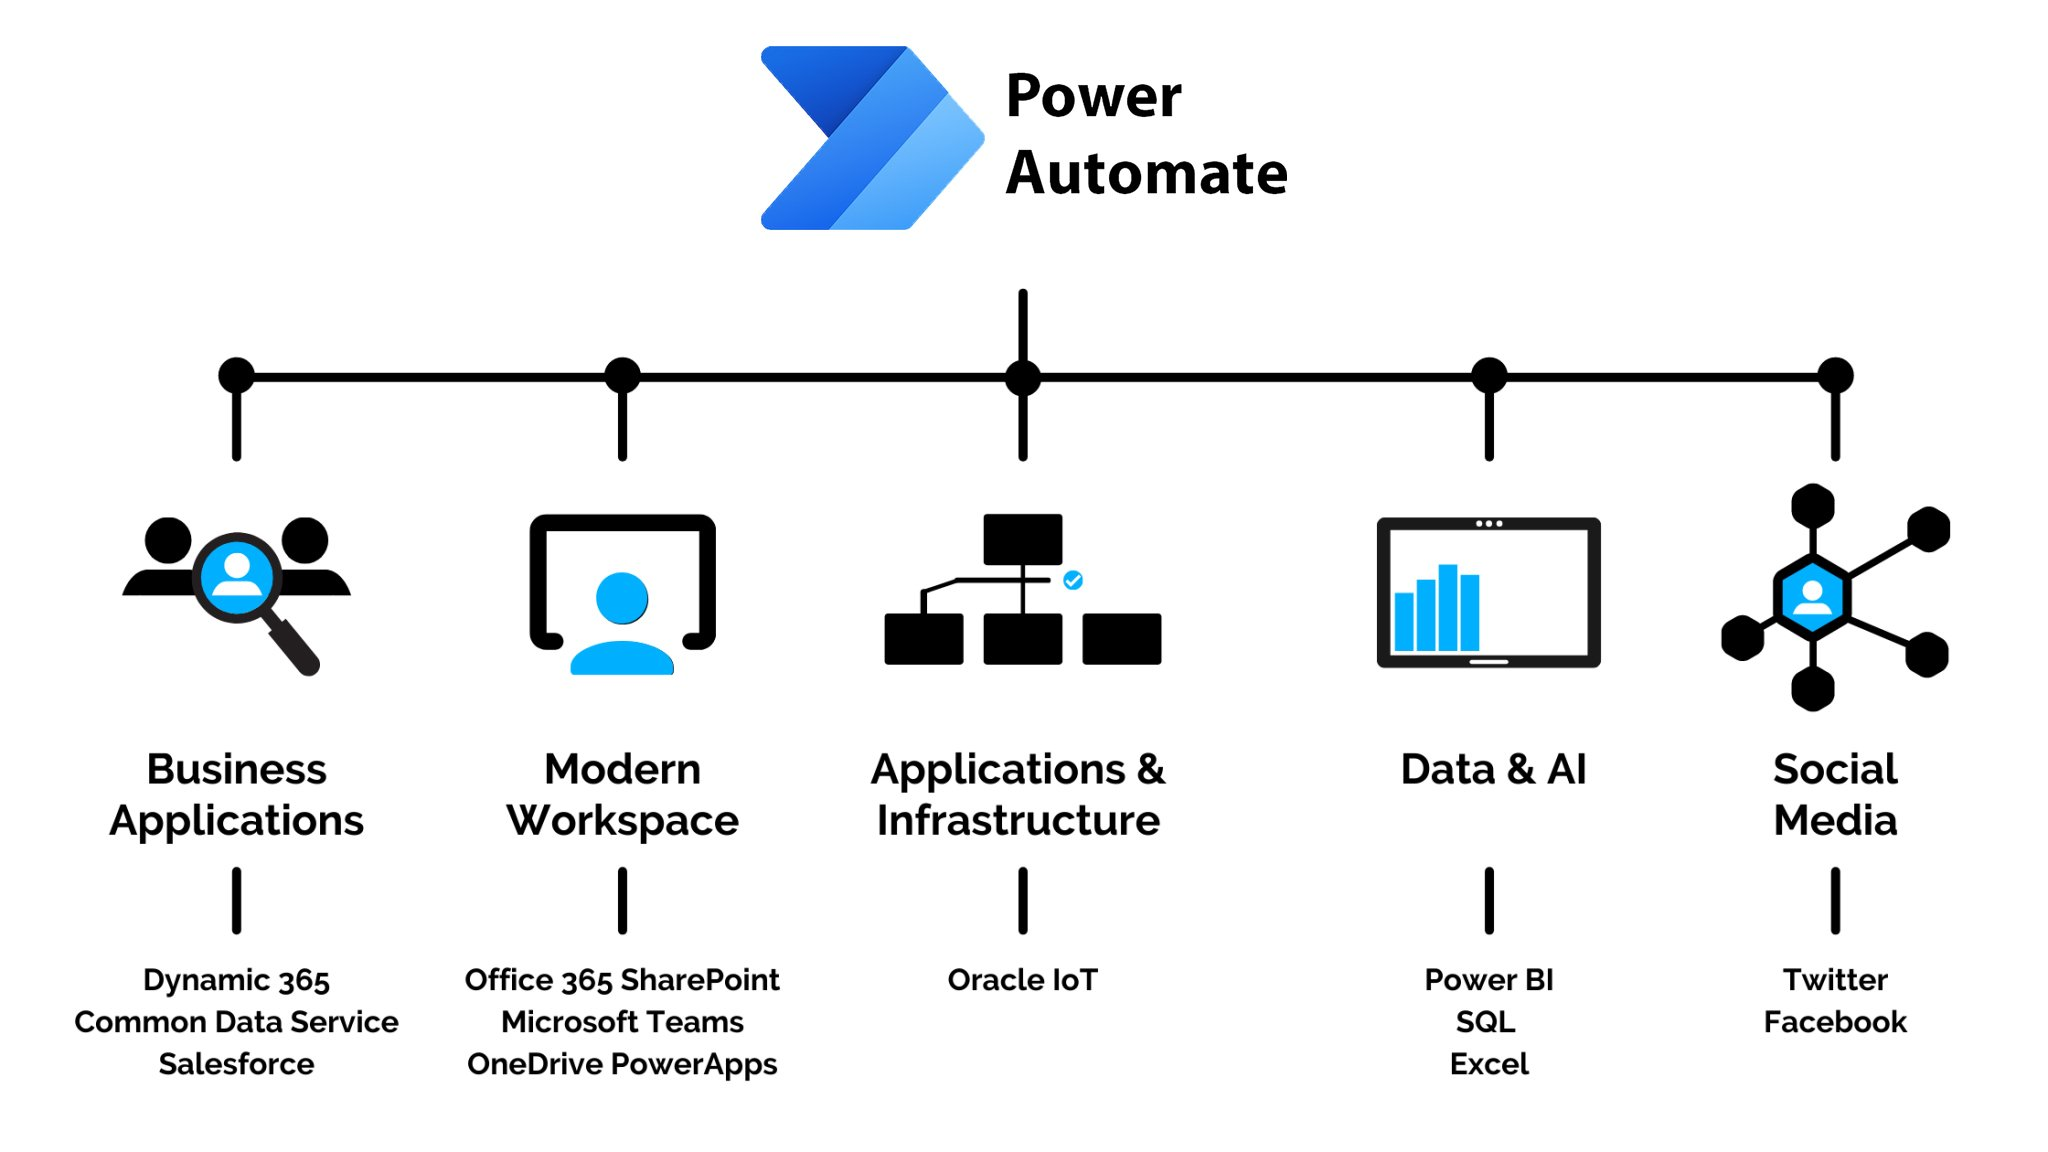
\includegraphics[width=0.48\textwidth]{images_pfe/power automate.jpg}
  \caption{Microsoft Power Automate interface used for orchestration interactions.}
  \label{fig:power_automate}
\end{figure}

\vspace{0.3cm}
\noindent\textcolor[HTML]{0066CC}{\textbf{3. Validation Layer}}

The specification validation runs by a defined service that uses Azure Functions, it takes the technical specification as input and executes the configured rules to return a validated report. It does not affect the conversation flow, which makes it deterministic and reproducible.

\begin{figure}[H]
  \centering
  
\includegraphics[width=0.48\textwidth]{images_pfe/azure function.png}
  \caption{Azure Functions interface used for validation interactions.}
  \label{fig:azure_functions}
\end{figure}

\vspace{0.3cm}
\noindent\textcolor[HTML]{0066CC}{\textbf{4. Data Management Layer}}

At this level the system utilizes several different data stores, which support governance and validation activities such as the conversational interface that uses structured data store, the enterprise document store (real time governance data and deliverables) and the configuration store (validation rules and templates).

\begin{figure}[H]
  \centering
  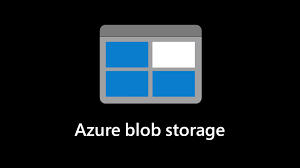
\includegraphics[width=0.48\textwidth]{images_pfe/Azure Storage.png}
  \caption{Azure Storage interface used for data management interactions.}
  \label{fig:azure_storage}
\end{figure}

\vspace{0.2cm}

To conclude, this combination of technologies enables LEON to orchestrate dialogues and automate processes, while allowing data to be accessed and validated through a single system. It complements the system specification and offers a flexible way to manage governance processes in an enterprise environment.

\subsection{\textcolor[HTML]{003D99}{Deployment Architecture (Multi-Environment)}}

LEON deployment strategy is centered around multi-environment where it is built, tested and released to production in a controlled and monitored way which is compatible with the Stellantis enterprise system. This process enables safe evolution of the system without compromising its reliability and controllability during the implementation.

Three main environments are used:\\

\vspace{0.2cm}
\noindent\textcolor[HTML]{0066CC}{\textbf{A. Development Environment (Dev)}}

Development Environment is an environment that allows for the fast prototyping and incremental development of new features. Within this environment the developers are able to design and test conversation flows, workflows, and validation logic without relying on production data. In essence, this is a sandbox in which to test and debug quickly.\\

\vspace{0.2cm}
\noindent\textcolor[HTML]{0066CC}{\textbf{B. Test Environment (Test)}}

The test environment is the staging environment used to run the implemented functions and ensure they work, prior to reaching the production environment. It is used in the process of testing scenarios and performing UAT (User Acceptance Testing).\\

\vspace{0.2cm}
\noindent\textcolor[HTML]{0066CC}{\textbf{C. Production Environment (Prod)}}

This is where LEON is installed and connected to Stellantis end users. This is the environment which can support verified configuration and fixed workflow. The environment where end users can use LEON governance services and validation functions.

\vspace{0.3cm}
\noindent\textcolor[HTML]{003D99}{\textbf{Environment Promotion Strategy}}

Promoted to environments carefully, configurations and work flows will be transported step by step to Development, to Test, then to Production. With this, we can allocate enough time to validation and testing, and do not have to work with untested components until the final users.

\vspace{0.3cm}

This multi environment architecture manages the evolution of system with safety as it segregates system into isolated environment on top of a shared data architecture. This approach will improve the deployment, maintain the system stability and allow a stepwise evolve of LEON without compromise on enterprise integrity.

% ═════════════════════════════════════════════════════════════════════════════
\section{\textcolor[HTML]{0066CC}{Governance Block Implementation}}
\label{sec:impl-governance}
% ═════════════════════════════════════════════════════════════════════════════

Users interact with LEON's Governance block to manage project components, roles, and responsibilities—all through natural conversation. Rather than switching between Excel spreadsheets, project management tools, and email, engineers simply ask LEON questions: ``Who is responsible for the brake system in J4U?'' or ``Update the DRE for the dashboard to John Smith.''

The Governance block connects three core components: (1) Copilot Studio manages the conversation and understands user intent, (2) Power Automate orchestrates the business logic and data updates, and (3) Excel spreadsheets on SharePoint store the governance data. This architecture works because it integrates with tools that Stellantis teams already use—there's no new system to learn.

This section details how five governance services function: how topics route conversations to the right handler, how LEON looks up component responsibilities, how it tracks project gates, how it updates assignments when engineers change roles, and how it manages document uploads to gate milestones.

\vspace{0.3cm}
\noindent\fbox{%
    \parbox{0.95\textwidth}{%
        \textcolor[HTML]{0066CC}{\textbf{Governance Services at a Glance:}} Users ask questions about project components, LEON queries Excel governance data through Power Automate, and responds conversationally. Updates are logged for compliance, and affected teams receive notifications automatically.
    }%
}
\vspace{0.3cm}

\subsection{\textcolor[HTML]{003D99}{Copilot Studio Topics and Conversation Design}}
\label{sec:impl-topics}

\subsubsection{Topic Architecture}

Topics are the core orchestration mechanism in Copilot Studio. Each governance service is mapped to one or more topics:

\begin{center}
\begin{tabularx}{0.95\textwidth}{|l|X|X|}
    \hline
    \textbf{Topic} & \textbf{User Query} & \textbf{Associated Functions} \\
    \hline
    \textbf{Who-is-Who Search} & ``Who is responsible for component [Component]?'' & Lookup flow trigger \\
    \hline
    \textbf{Gate Status} & ``What is the current gate for [Component]?'' & Gate metadata retrieval \\
    \hline
    \textbf{Update Responsible} & ``Update responsible for [Component] to [New Name].'' & Update flow with RBAC validation \\
    \hline
    \textbf{Upload Deliverable} & ``Upload my specification for gate [Gate].'' & File attachment and SharePoint routing \\
    \hline
    \textbf{Workload Management} & ``Show me my workload.'' & Assignment retrieval and updates \\
    \hline
    \textbf{Send Notification} & ``Send a reminder to [actor].'' & Email trigger via Power Automate \\
    \hline
    \textbf{Escalate} & Unresolved queries & Human support team escalation \\
    \hline
\end{tabularx}
\end{center}

\subsubsection{Knowledge Base Integration}

The Copilot Studio knowledge base organizes governance data into structured repositories:

\begin{itemize}
    \item[\quad\textbullet] \textcolor[HTML]{003D99}{\textbf{Who-is-Who dataset}} : Excel file with Project, Component, Responsible Name, Responsible Email, Role, Active columns.
    \item[\quad\textbullet] \textcolor[HTML]{003D99}{\textbf{Gate metadata}} : Project, Component, Current Gate, Gate Entry Date, Expected Exit Date, Gate Owner.
    \item[\quad\textbullet] \textcolor[HTML]{003D99}{\textbf{Validation guidelines}} : Acceptance criteria documentation per gate level.
    \item[\quad\textbullet] \textcolor[HTML]{003D99}{\textbf{SharePoint data connectors}} : Real-time links to governance lists and tables for live queries.
\end{itemize}

\noindent Entity extraction via NLU processes user utterances and queries these knowledge sources to provide contextual answers.

\subsection{\textcolor[HTML]{003D99}{Implementation: Who-is-Who Responsible Lookup}}
\label{sec:impl-whoiswho}

\subsubsection{Objective and Scope}

The Who-is-Who responsible lookup service can be used by the user to discover the person accountable for a component within a project using query (via excel) into the governance data source. This can be triggered conversationaly through Copilot studio by using Power Automate flows and will provide an accountable person identifier or an error code (managed through conversational invocation) as output.
\subsubsection{Where the Data Lives}

LEON counts on Stellantis governance teams which used to be responsible for mapping component responsibility in Excel. Therefore, instead of building up a database, LEON is just linked to the excel on SharePoint. This implies that:
\begin{itemize}
    \item Same modification done by the Governance engineers as it has been before
    \item LEON auto-reads changes automatically with no workflow.
    \item Permissions are inherited. If one user is allowed to change the spreadsheet, then this user can start an update through LEON.
    \item Teams will not play around with new tools. It‘s just that the information becomes readily available.
\end{itemize}

\begin{figure}[H]
    \centering
    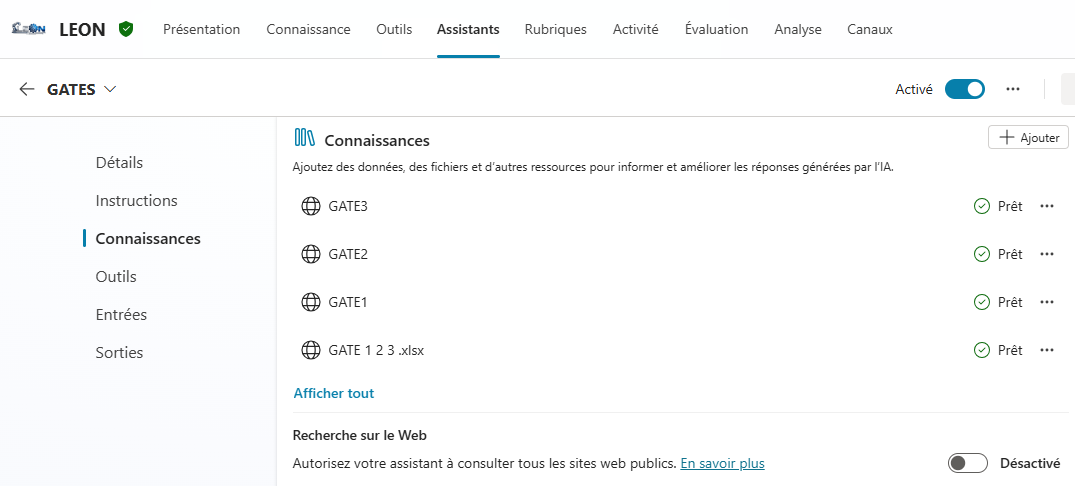
\includegraphics[width=0.5\textwidth]{images_pfe/knowledge gate.png}
    \caption{Who-is-Who Excel structure: Each project gets a sheet (J4U, SP1-P1H, etc.), components are rows, roles are columns.}
    \label{fig:w1-dataset-structure}
\end{figure}

\noindent\textbf{File Organization:}

\begin{itemize}
    \item[\quad\textbullet] \textbf{One Excel file}: The workbook is the single source for governance data.
    \item[\quad\textbullet] \textbf{Multiple sheets}: Each sheet has the name of the corresponding project (e.g. “J4U”, “SP1-P1H”, “X2Y”). New projects should be associated with a new sheet.
    \item[\quad\textbullet] \textbf{Sheet structure}: Each sheet employs identical tabular layout for consistency:
    \begin{itemize}[leftmargin=0.5cm]
        \item \textcolor[HTML]{003D99}{\textbf{First column}} :  Is a “Component” header, component ids that are unique within the project.
        \item \textcolor[HTML]{003D99}{\textbf{Subsequent columns}} :  Organization role headers (i.e. “DRE”, “DL”, “Pilot”, “Global CTE”) and person names in the cells.
        \item \textcolor[HTML]{003D99}{\textbf{Header row}} : The role name should be in the first row of each sheet and the role may differ among each:
    \end{itemize}
    \item[\quad\textbullet] \textbf{Cell values}: In the intersection of component row and role column name of responsible person should be displayed if only one. If there are more than one responsible persons, it has to be separated using either “/” or “,” based on how it is written in the table.
    \item[\quad\textbullet] \textbf{Empty cells}: Show that there is no accountable person for the specific combination of component-role.
    \item[\quad\textbullet] \textbf{Dynamic identification}:  Order of columns and role names can be identified dynamically per sheet and is not fixed, therefore giving the flexibility.
\end{itemize}

\noindent The excel multiple tab structure is extremely flexible, new projects are created by adding new sheets to the spreadsheet and new roles can be created by adding more columns of data to the table.



\subsubsection{How the Lookup Works: A Real Example}

An engineer may ask (e.g. ” DRE of brake system for the J4U project ? ”). The answer LEON gives :

\begin{enumerate}
\item \textbf{Understands intent:} Copilot NLU finds three attributes that are the J4U project, the brake system component and the role of DRE.
\item \textbf{Finds the project sheet:} LEON checks if J4U matches any sheet name in the Excel file
\item \textbf{Locates the component row:} In the Component column, LEON seeks out “brake system” (or similar, if not exactly).
\begin{figure}[H]
    \centering
    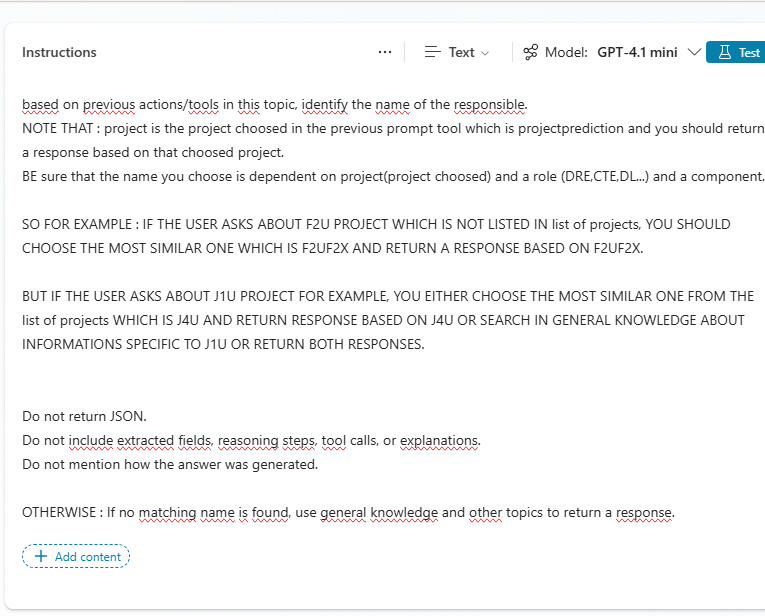
\includegraphics[width=0.85\textwidth]{images_pfe/name search.png}
    \caption{Component search workflow: Locating component row in Excel.}
    \label{fig:w4-lookup}
\end{figure}
\item \textbf{Finds the role column:} Looks across the first row for the DRE column header
\item \textbf{Returns the answer:} LEON reads the cell at the intersection and finds the responsible engineer's name
\end{enumerate}


\textbf{Why this design matters:} Engineers doesn‘t need to provide the exact string in Excel because there is a phase of normalization (case insensitive, trimming leading and trailing spaces) that handles all inputs of the users. The tolerance is good for user as there is less confusion and less question.

\subsubsection{Handling Project Name Ambiguity}

Not all of the users and enginners remembers the exact project codes or names. While testing the pilot program we had discover that:

\begin{itemize}
\item The variation of cases (”J4U” vs “j4u”, etc)
\item Some institutions (or engineers) write abbreviations (``J4'' instead of ``J4U'')
\item Many also use codenames or nicknames for projects rather than their official designation.
\end{itemize}

To handle this, we implemented a two-step matching process:

\textbf{Step 1: Exact Match (Case Insensitive)}  
LEON converts the user input to lower case and compares it with the names of the excel sheets. If there is sheet called J4U and the user enters either j4u or J4u, there is a matching case.

\textbf{Step 2: Similarity Fallback}  
Similarity fallback if there are no exact matches, we are looking for partial matches. The engineer who gives “the automotive project four” to the system, will not be able to find the “J4U” name. We don‘t want to filter the engineer but assist him. Copilot, using NLU, will search and provide him the closest matching name and will suggest it by asking him: “did you mean the J4U project ?” to prevent any potential escalation.

\subsubsection{Finding the Right Cell}

Upon approval of the project sheet, LEON attempts to find the component and the role in it. This step might seem straightforward at first, but has some practical drawbacks:


\begin{itemize}
\item \textbf{Component naming varies:} In one project, the engineer uses ‘extermirrors’, the other one use ‘ext.mirrors’ or just ‘MirrorSystem’. We accept missing spaces and ignore case while matching, and calculate the similarity score
\item \textbf{Role columns differ by project:}  In J4U, there are “DRE”, “Pilot”, and “CTE”, whereas in SP1-P1H there are “DL”, “Global CTE”, and “Quality Lead”. The headers will be dynamically read in, rather than hard coded.
\item \textbf{Multiple responsibilities:} There are situations where one cell is responsible for more than one individual; such as “Jane Smith / John Doe”. LEON presents back the two individuals to the user.
\end{itemize}

\subsubsection{Error Handling and Fallback}

\noindent The service produces the following error conditions:

\vspace{0.15cm}

\begin{tabularx}{0.95\textwidth}{|l|X|}
    \hline
    \textbf{Error} & \textbf{What Went Wrong} \\
    \hline
    \texttt{PROJECT NOT FOUND} & User said a project name that doesn't exist. Copilot suggests available projects. \\
    \hline
    \texttt{COMPONENT NOT FOUND} & Component not in the sheet we return this rather than guessing. \\
    \hline
    \texttt{ROLE NOT FOUND} & Requested role (e.g., ``CEO'') doesn't exist in that project's columns. \\
    \hline
    \texttt{RESPONSIBLE NOT ASSIGNED} & Cell is empty ,no one assigned to that component role yet. \\
    \hline
    \texttt{DATASET UNAVAILABLE} & SharePoint is down or network issue. User retries later. \\
    \hline
    \texttt{UNAUTHORIZED} & User lacks permission to read that project. Security enforced at Excel level. \\
    \hline
\end{tabularx}





\subsubsection{Output Format}

Who-is-Who lookup is showing one of the outcomes only, it depends upon execution.

\begin{itemize}
    \item[\quad\textbullet] \textbf{Success}: If it is a success, server sends to client cell contents (a cell, one or many names) exactly like it is saved in the cell in excel (without any pre-treatment).
    \item[\quad\textbullet] \textbf{Error}: When the lookup fails the function returns an error code such as for instance \texttt{PROJECT NOT FOUND} which will be mapped by Copilot Studio into a conversational response.
    \begin{figure}[H]
    \centering
    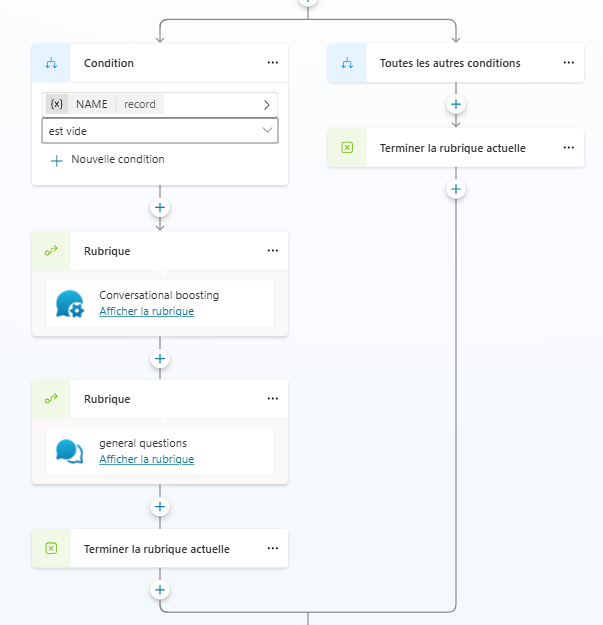
\includegraphics[width=0.9\textwidth]{images_pfe/condition who.png}
    \caption{Error condition handling workflow: Decision tree for error scenarios in Who-is-Who lookup.}
    \label{fig:w5-error-condition}
\end{figure}
\end{itemize}



\subsection{\textcolor[HTML]{003D99}{Implementation: Gate Status Retrieval}}
\label{sec:impl-gatestatus}

\subsubsection{Why Gate Status Matters}

The development process of an automotive product involves gates : Gate 1 for concept, Gate 2 for detail design, Gate 3 for pre-production. The engineers will want to know: ” Has the brake system reached Gate 2 ? ”. This then determines the relevant design reviews that are needed.

While Who is Who is nothing more than a lookup on an excel table, gate status is kept in documents. When a component passes through a gate the spec is stored in a SharePoint folder, namely, ’/LEON-Governance/J4U/Gate-2/Brake-System/’. Then Gate Status is determined by looking through the folders where a particular document resides.

\textbf{Why this approach?} The gates are a governance mark used by Stellantis. we are reading files, so we would not be inventing a new system to be updated if metadata were separated from the other parts of information. The guess is that gate 3 is skipped or served much more rapidly if gate 3 is present in the catalog but not gate 2.

\subsubsection{Data Source}

The status of a gate is inferred via a knowledge structure in the documents with three gate levels:

\begin{figure}[H]
    \centering
    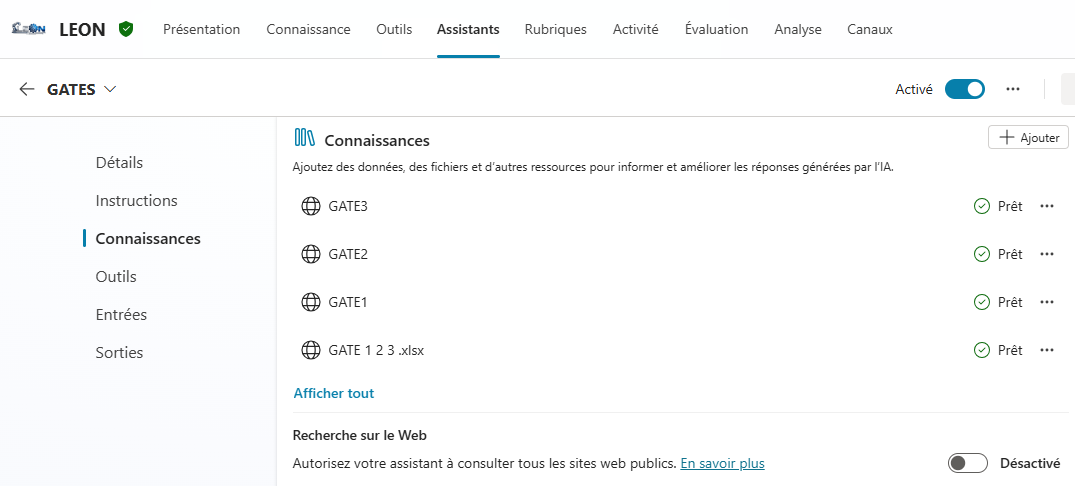
\includegraphics[width=0.85\textwidth]{images_pfe/knowledge gate.png}
    \caption{Knowledge base organization: Gate 1, Gate 2, and Gate 3 document repositories.}
    \label{fig:gate-knowledge-structure}
\end{figure}

\begin{itemize}
    \item[\quad\textbullet] \textbf{GATE1}: Knowledge source/folder contains documents associated with Gate 1 deliverables.
    \item[\quad\textbullet] \textbf{GATE2}: Knowledge source/folder contains documents associated with Gate 2 deliverables.
    \item[\quad\textbullet] \textbf{GATE3}: Knowledge source/folder contains documents associated with Gate 3 deliverables.
\end{itemize}

\subsubsection{How Documents Signal Gate Progress}

Project documentation on Stellantis is stored on SharePoint and organized by project, then by gate. Upon the brake system reaching Gate 2, the specification is placed on ”/LEONGovernance/J4U/GATE2/Brake-System/”. LEON is responsible for identifying which gate folders the component specification shall be forwarded:
\begin{itemize}
    \item[\quad\textbullet] \textbf{GATE1}: Concept documents for components that were approved for design phase
    \item[\quad\textbullet] \textbf{GATE2}: Design documents for components that passed detailed design review
    \item[\quad\textbullet] \textbf{GATE3}: Pre-production documents for components that are ready for manufacturing
\end{itemize}

When there are documents relating to the GATE2 Brake System, but not for the GATE3 component, the reasoning applied is that the component is in GATE2. When the GATE1 & GATE3 exist, but GATE2 is empty, the reasoning is that the component skipped GATE2, (or has an accelerated review process).
\vspace{0.2cm}

\noindent\textbf{Understanding the Query:}

For the query: “What gate is the suspension system at in J4U?”, Copilot NLU would return: project = J4U, component = suspension system. Both would be normalized to, say: “j4u” normalized to “J4U”, “suspension system”, and “suspension subsystem”. Using case insensitive prefix matching and substring search the parser can map all those strings appropriately.
\subsubsection{How LEON Finds the Gate}

The search process is straightforward:

\begin{enumerate}
    \item \textbf{Check Gate 3 first} (most advanced): Is there a file in ‘LEON Governance/J4U/GATE3/Suspension-System/’? Yes, your component is in Gate 3.
    \item \textbf{If not, check Gate 2}: If not, then try Gate 2: Is ”/“LEON-Governance/J4U/GATE2/Suspension-System/” with documents? if yes Gate 2.
    \item \textbf{If not, check Gate 1}: Otherwise: check Gate 1, find whether ’/LEON-Governance/J4U/GATE1/Suspension-System/’ exists in documents or not. If it exists, Gate 1.
    \item \textbf{If nothing found}: Component not at a recorded gate. LEON tells user: ” The suspension system has not yet been formally recorded at a gate”.
\end{enumerate}

\begin{figure}[H]
    \centering
    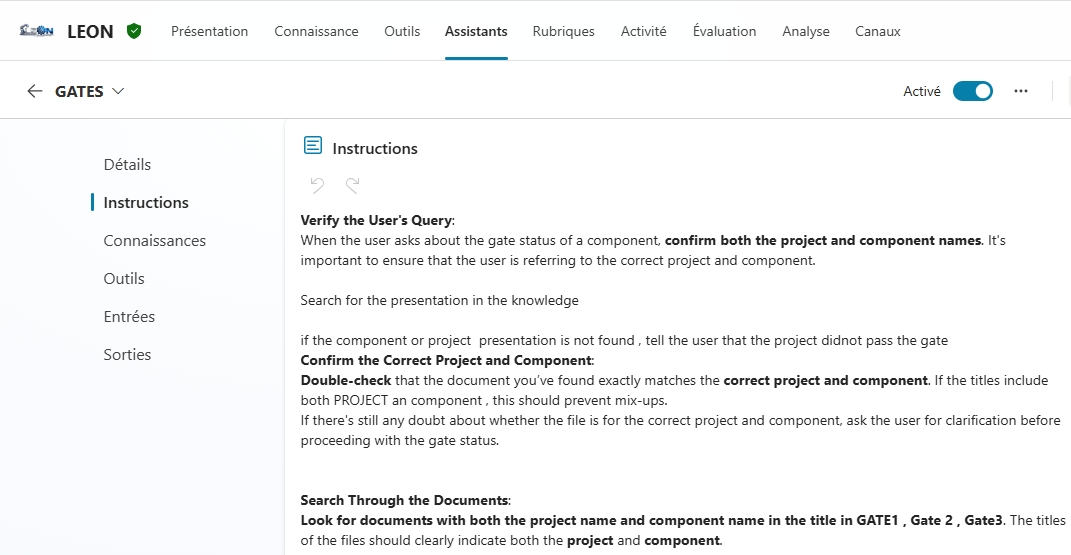
\includegraphics[width=0.45\textwidth]{images_pfe/gate1.png}
    \hfill
    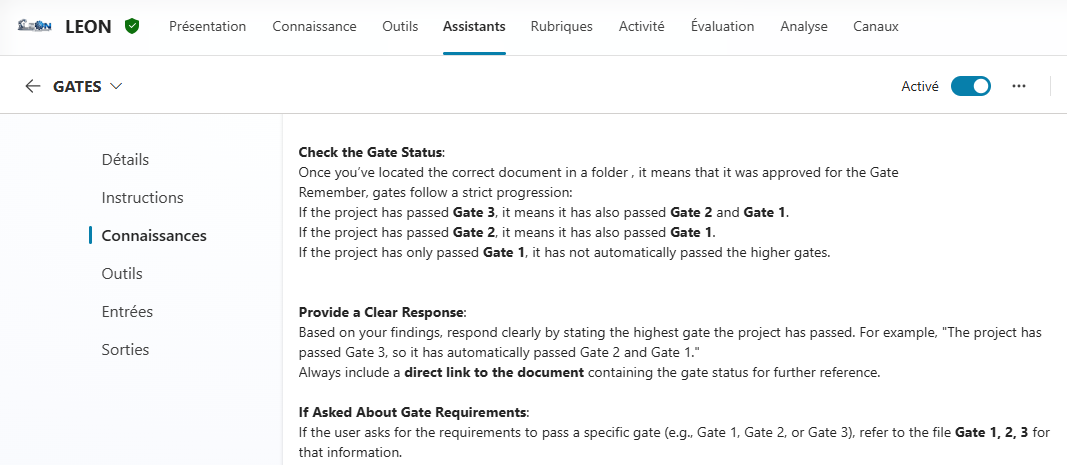
\includegraphics[width=0.45\textwidth]{images_pfe/gate2.png}
    \caption{Gate detection workflow: (left) document search across gate repositories; (right) highest gate level identification.}
    \label{fig:gate-detection-workflow}
\end{figure}

This document outlines the detection method that will be based on asserting that gate status is representative of the knowledge bases uploaded objects and stored objects that have not activated some other attribute to denote metadata.

\subsubsection{Error Handling and Fallback}

The service produces the following error or incomplete-result conditions:

\vspace{0.15cm}

\begin{tabularx}{0.95\textwidth}{|l|X|}
    \hline
    \textbf{What Happens} & \textbf{What LEON Does} \\
    \hline
    \texttt{PROJECT NOT FOUND} & Project doesn't exist in documents. LEON suggests alternatives: ``Did you mean J4U or SP1-P1H?'' \\
    \hline
    \texttt{COMPONENT NOT FOUND} & Component name doesn't match anything in that project. LEON asks: ``Which component? I can search available ones.'' \\
    \hline
    \texttt{NO GATE REACHED} & Valid project and component, but no gate documents found yet. LEON responds: ``The brake system hasn't reached a gate yet.'' \\
    \hline
    \texttt{KNOWLEDGE BASE UNAVAILABLE} & SharePoint is down or network issues prevent document search. LEON says: ``I can't access the gate documents right now. Try again in a moment.'' \\
    \hline
    \texttt{AMBIGUOUS MATCH} & Multiple documents with similar names (e.g., brake-system-v1, brake-system-final). LEON asks user to clarify which one. \\
    \hline
\end{tabularx}

\vspace{0.2cm}

\noindent For any error condition, Copilot Studio routes to fallback topic (Escalate) or requests user clarification.

\subsubsection{Output Format}

The Gate Status service returns a conversational response indicating:

\begin{itemize}
    \item[\quad\textbullet] \textbf{Success}: Identified at gate level (GATE1, GATE2 or GATE3) in a natural language. Example: Seat Actuator component in the project of XEV has reached GATE2 based on documents in the knowledge base.
    \item[\quad\textbullet] \textbf{Incomplete}: Clarification that we have not reached a documented gate. Example: Seat Actuator component in the project of XEV has not yet reached a documented gate.
    \item[\quad\textbullet] \textbf{Error}: error message and suggestions for next steps (refined search, confirmation, escalation)
\end{itemize}

\paragraph{Extension: Gate Document Upload (In Development)}

A further functionality that is under development and that allows the user to upload files to a particular gate:

\begin{enumerate}
    \item \textcolor[HTML]{003D99}{\textbf{User input}} : Upload deliverable for this excat component in this project inside the gate1. (with file attachment)
    \item \textcolor[HTML]{003D99}{\textbf{Copilot processing}} : extracts project, component, gate level, and file.
    \item \textcolor[HTML]{003D99}{\textbf{Validation}} : for each one of the three parameters (project, component, gate) check that it is well specified and that it exists.
    \item \textcolor[HTML]{003D99}{\textbf{Storage}} : The document should be uploaded in the correct gate repository (more specific folder GATE1, GATE2, GATE3 under the Knowledge Source). A file will be registered with its metadata such as Uploader, Creation date, Project, Component and Gate.
    \item \textcolor[HTML]{003D99}{\textbf{Logging}} : log the upload event to audit trail (timestamp, user identity, file, gate, status).
    \item \textcolor[HTML]{003D99}{\textbf{Response}} : confirm successful upload with file reference and gate location.
\end{enumerate}

\textbf{Note:} This feature (upload) is not yet implemented but it is scheduled for next release so that the components are sent to gates by the user who manage files by the LEON.

\subsection{\textcolor[HTML]{003D99}{Implementation: Responsible Assignment Update}}
\label{sec:impl-responsible-update}

\subsubsection{When Responsibilities Change}

Product development teams evolve. When a responsible moves to a new role, a new responsible takes over as his role for a specific componenet. When a design review is assigned to a new engineer, that person’s name needs to appear in the governance record.

Instead of Governance teams updating themselves in excel: find sheet, row, and column, added new name, saved file, e-mailed. With LEON: Updated the DRE for dashboard component in J4U to Sarah Chen and updated right away. It also logs who and when made the update, and what the change actually was, useful for auditable history of development.

\subsubsection{Where Updates Happen}

Updates are made to the same Excel file where Who-is-Who queries to. File has one sheet per project (J4U, SP1-P1H) where each component is a row and in each role we have a column. Updating DRE for the brake system to Sarah Chen, it means we update one cell in the J4U excel file, in the row brake system and in the column DRE. LEON is doing it via Power Automate excel connector, which has complete write permissions to the shared governance file.

\textbf{Why this matters:} All this information is readily available from the governance groups. We are not building yet another place to try and keep in sync. Updates to LEON are visible immediately when you open the Excel, and if a governance engineer makes a change directly into the Excel it will show up in the following query.

\subsubsection{What Information LEON Needs}

To make an update for the name of a responsible in a project, LEON needs four pieces of information:

\begin{itemize}
    \item[\quad\textbullet] \textbf{Project}: Which project? (J4U, SP1-P1H, etc.), the user should choose the project sheet to update.
    \item[\quad\textbullet] \textbf{Component}: Which component? (Brake System, Dashboard, etc.), the user should choose the component to update.
    \item[\quad\textbullet] \textbf{Role}: Which role? (DRE, Pilot, CTE, etc.), the user should choose the role to update.
    \item[\quad\textbullet] \textbf{New Name}: Who is responsible now? The user should provide the new name of the responsible.
\end{itemize}

In case the article is missing Copilot asks the user to provide the missing information. Similarly to the Who-is-Who service LEON is not sensitive to format.

\subsubsection{How the Update Happens}

This is how LEON processes the request of an engineer asking for ‘Update the DRE for External mirrors in J4U to John Doe’:
\begingroup
\setlength{\intextsep}{6pt}
\setlength{\textfloatsep}{6pt}
\captionsetup[figure]{skip=4pt}
\begin{enumerate}[topsep=2pt,itemsep=4pt,parsep=0pt]
    \item \textbf{Extract the request}: Copilot NLU understands project=J4U, component=External mirrors, role=DRE, new person=John Doe
\item \textbf{Confirm the project}: If J4U is clear, proceed. If ambiguous, Copilot asks which project.
\item \textbf{Suggest matching components}: LEON will find parts in J4U sheet in ‘Search’ window with words “External mirrors” (for example “External mirrors”, “Mirror assembly”, “Ext mirrors”). Engineer will select a proper one.
    \begin{figure}[H]
    \centering
    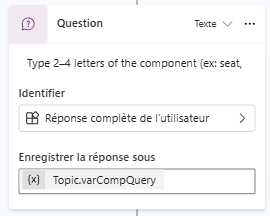
\includegraphics[width=0.4\textwidth]{images_pfe/Component input.png}
    \caption{Component input: User enters partial name; system prepares suggestion list.}
    \label{fig:component-input}
\end{figure}
\item \textbf{Show available roles}: For J4U, available roles are DRE, Pilot, CTE. Engineer confirms: ``Yes, DRE.''
    \begin{figure}[H]
    \centering
    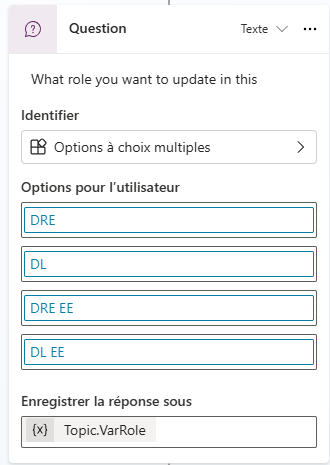
\includegraphics[width=0.4\textwidth]{images_pfe/question role.png}
    \caption{Role selection: User selects from available roles.}
    \label{fig:role-selection}
\end{figure}
\item \textbf{Confirm the change}: LEON prompts: Do you want to Update External mirrors (J4U) DRE from Jane Smith to John Doe? Yes or No
    \begin{figure}[H]
    \centering
    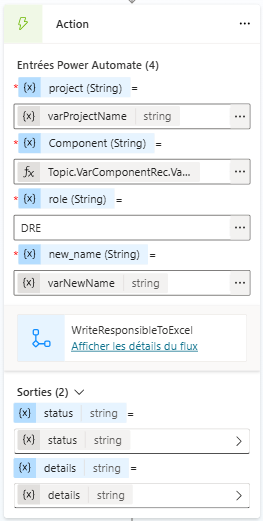
\includegraphics[width=0.35\textwidth]{images_pfe/update name1.png}
    \caption{Update execution: User confirms the assignment update.}
    \label{fig:update-execution}
\end{figure}
\item \textbf{Make the change}: Power Automate opens the Excel file, then it locates the cell (row External mirrors and column DRE in J4U) and writes John Doe in it, saves the file, and logs that modification.
    \begin{figure}[H]
    \centering
    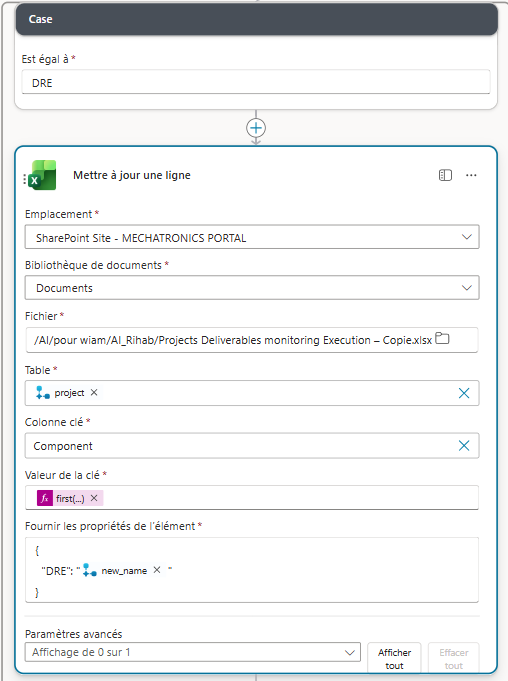
\includegraphics[width=0.4\textwidth]{images_pfe/update name2.png}
    \caption{Update execution: Cell value update in Excel.}
    \label{fig:update-write}
\end{figure}
\item \textbf{Confirm to user}: LEON confirms: ``Done. John Doe is now DRE for External mirrors in J4U.''
\end{enumerate}
\endgroup
\subsubsection{Error Handling}

What can go wrong when updating assignments:

\vspace{0.15cm}

\begin{tabularx}{0.95\textwidth}{|l|X|}
    \hline
    \textbf{What Happens} & \textbf{What LEON Does} \\
    \hline
    \texttt{PROJECT NOT FOUND} & Project name doesn't match any sheet. LEON suggests available projects. \\
    \hline
    \texttt{COMPONENT NOT FOUND} & Component doesn't exist in that project. LEON lists available components. \\
    \hline
    \texttt{ROLE NOT FOUND} & Role name doesn't exist in that project (e.g., CEO for J4U). LEON shows available roles. \\
    \hline
    \texttt{INVALID NEW NAME} & New name is empty or invalid. LEON asks: Who should be assigned? \\
    \hline
    \texttt{UNAUTHORIZED} & User lacks write permission on the Excel file. LEON says: You can't modify this assignment. \\
    \hline
    \texttt{DATASET UNAVAILABLE} & SharePoint is down or Excel file can't be accessed. LEON says: Can't access Excel right now. Try again later. \\
    \hline
    \texttt{WRITE FAILURE} & Excel write fails (file locked, quota exceeded). LEON escalates: Update failed. Contact IT. \\
    \hline
\end{tabularx}

\vspace{0.2cm}


\subsubsection{Output Format}

The response given by the Responsible Assignment Update service to the Copilot Studio at every attempt to update is presented as follows (see Figure~5.14).
 \begin{figure}[H]
    \centering
    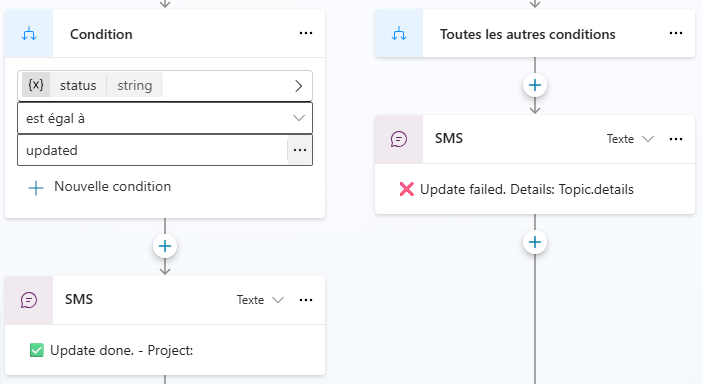
\includegraphics[width=0.4\textwidth]{images_pfe/update name.png}
    \caption{Update execution: Final confirmation and result to user.}
    \label{fig:update-result}
\end{figure}

\begin{itemize}
    \item[\quad\textbullet] \textbf{Success case}: 
The success path explicitly includes the step that the change was made while indicating the old responsible and the new one to be used during the process. The data returned consists of: \texttt{status=updated}, the \texttt{old responsible}, the \texttt{new responsible} and a timestamp in the ISO-8601 format. Copilot Studio presents a small confirmation message that summarizes the updated project, the component and the role to be affected by the update.
    \item[\quad\textbullet] \textbf{Error case}: 
    In the case of failure of update, the service will respond with error response where status will be with the error code (COMPONENT NOT FOUND, UNAUTHORIZED, etc.) and short details field. Copilot Studio will render a user friendly error message and present with the next action to perform (Retry with updated data, Specify, escalate...).
\end{itemize}





\subsection{\textcolor[HTML]{003D99}{Implementation: Send Notification and Email}}
\label{sec:impl-notification}

\subsubsection{Objective and Scope}

The Send Notification and Email service enables users to communicate with project stakeholders through structured email messages. The service supports two operational modes: (1) draft mode, where email messages are prepared for review without sending, and (2) send mode, where messages are immediately transmitted to recipients. The service integrates recipient resolution via Azure Active Directory (AAD) directory lookup, message composition via user input or predefined templates, and email transmission via the Microsoft Outlook connector. \textbf{All emails are user-generated or template-based;} the system does NOT perform autonomous message composition or AI-generated content. All email operations are logged for audit and compliance purposes.

\subsubsection{System Architecture}

The email service is implemented through the following integrated components:
 \begin{figure}[H]
    \centering
    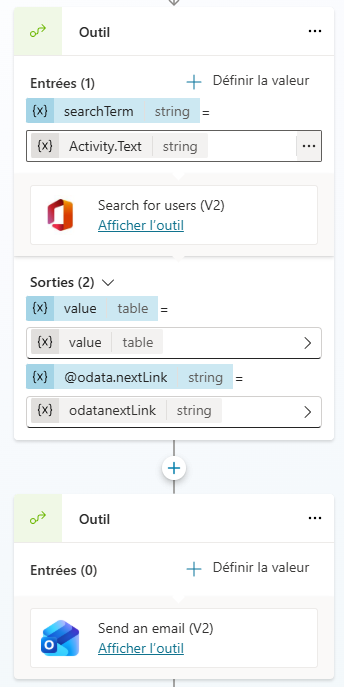
\includegraphics[width=0.4\textwidth]{images_pfe/email.png}
    \caption{Email service architecture overview.}
    \label{fig:email-architecture}
\end{figure}
\begin{itemize}
    \item[\quad\textbullet] \textbf{Copilot Studio}: Conversational interface for user intent detection and message orchestration.
    \item[\quad\textbullet] \textbf{Power Automate}: Workflow execution engine that coordinates recipient resolution, validation, and transmission.
    \item[\quad\textbullet] \textbf{Azure Active Directory (AAD) connector}: Provides user directory search via ``Search for users (V2)'' action for recipient resolution.
    \item[\quad\textbullet] \textbf{Microsoft Outlook connector}: Handles email transmission via [Company] mail service.
    \item[\quad\textbullet] \textbf{Copilot audit logs}: Records all email operations for compliance and traceability.
\end{itemize}

\subsubsection{Input Processing}

The email service accepts the following user inputs:
 \begin{figure}[H]
    \centering
    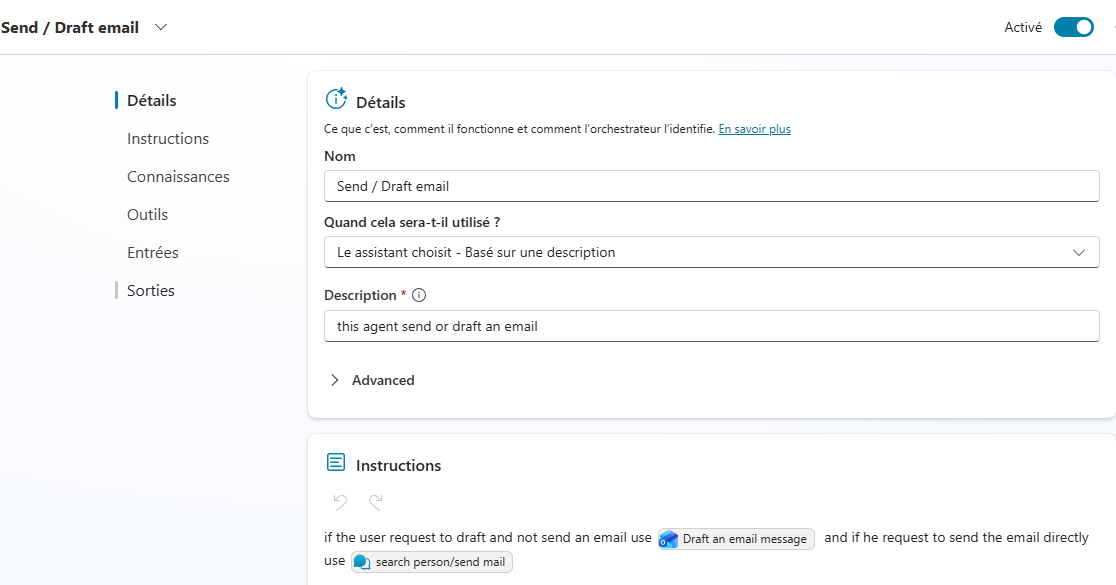
\includegraphics[width=0.4\textwidth]{images_pfe/email assistant.png}
    \caption{Email service architecture overview.}
    \label{fig:email-architecture}
\end{figure}
\noindent\fbox{%
    \parbox{0.95\textwidth}{%
        \textbf{User Input Parameters:}
        \begin{itemize}[leftmargin=0.3cm, itemsep=0.15cm]
            \item \textbf{Operation mode}: ``draft'' or ``send''
            \item \textbf{Recipient}: Name, email partial, or keyword for directory lookup
            \item \textbf{Subject}: Email subject line
            \item \textbf{Body}: Message content provided by user or selected from predefined templates
            \item \textbf{Context (optional)}: Project, component, or assignment reference for template variable substitution
        \end{itemize}
    }%
}

\vspace{0.2cm}

\noindent\textbf{Input Processing Steps:}

\begin{enumerate}
    \setlength{\itemsep}{0.1cm}
    \setlength{\leftmargin}{0.5cm}
    \item \textbf{Conversational capture}: User provides email request through Copilot Studio natural language interface. Example: ``Send an email to John Doe about component X4'', or ``Draft a message to the DRE responsible for this component.''
    \item \textbf{Intent detection}: Copilot NLU analyzes user utterance to determine:
    \begin{itemize}
        \setlength{\leftmargin}{0.7cm}
        \item Operation intent: draft or send
        \item Recipient specification (name, keyword, or role)
        \item Message content (subject, body, or template reference [à préciser])
    \end{itemize}
    \item \textbf{Validation}: System checks that required parameters (mode, recipient, subject, body) are provided. Missing inputs trigger Copilot clarification requests.
\end{enumerate}

\subsubsection{Recipient Resolution}

Recipient resolution is handled by the Power Automate ``Search for users (V2)'' action, which queries Azure Active Directory:

\begin{enumerate}
    \setlength{\itemsep}{0.1cm}
    \setlength{\leftmargin}{0.5cm}
    \item \textbf{User query input}: Recipient identifier from user (name, email partial, or keyword).
    \item \textbf{AAD directory search}: Power Automate invokes ``Search for users (V2)'' with the user query.
    \item \textbf{Match result processing}:
    \begin{itemize}
        \setlength{\leftmargin}{0.7cm}
        \item \textbf{Exact single match}: Recipient email address is extracted and confirmed.
        \item \textbf{Multiple matches}: Copilot presents matching users as a selectable list; user selects the correct recipient.
        \item \textbf{No matches}: Return \texttt{USER\_NOT\_FOUND}; Copilot requests clarification or alternative recipient specification.
    \end{itemize}
    \item \textbf{Email extraction}: Confirmed recipient email address is extracted and passed to the execution logic.
\end{enumerate}

\noindent This approach ensures that emails are sent to verified directory identities, reducing delivery failures and incorrect recipient issues.

\subsubsection{Execution Logic}

Once recipient and message parameters are confirmed, the system executes the email operation:

\vspace{0.15cm}

\noindent\textbf{Case A: Draft Mode (Prepare without Send)}

\begin{enumerate}
    \setlength{\itemsep}{0.1cm}
    \setlength{\leftmargin}{0.5cm}
    \item \textbf{Email composition}: System assembles email message with:
    \begin{itemize}
        \setlength{\leftmargin}{0.7cm}
        \item \texttt{to}: Recipient email address (resolved)
        \item \texttt{subject}: Subject line from user input
        \item \texttt{body}: Message body from user input or template [à préciser]
    \end{itemize}
    \item \textbf{No transmission}: Email draft is NOT sent; it is retained in-memory or stored in [à préciser: temporary location].
    \item \textbf{Draft preview}: System displays email preview to user for review:
    \begin{center}
        \textbf{From:} [System sender] \\
        \textbf{To:} [Recipient name] $<$[recipient@email.com]$>$ \\
        \textbf{Subject:} [Subject line] \\
        \rule[0.5ex]{\textwidth}{0.5pt} \\{}[Message body preview]
    \end{center}
    \item \textbf{User action}: User reviews draft and selects:
    \begin{itemize}
        \setlength{\leftmargin}{0.7cm}
        \item ``Send'' (transitions to Case B)
        \item ``Edit'' (return to input for modification)
        \item ``Cancel'' (discard draft)
    \end{itemize}
\end{enumerate}

\vspace{0.15cm}

\noindent\textbf{Case B: Send Mode (Direct Transmission)}

\begin{enumerate}
    \setlength{\itemsep}{0.1cm}
    \setlength{\leftmargin}{0.5cm}
    \item \textbf{Flow trigger}: Copilot invokes Power Automate flow ``Flow-Send-Email'' with parameters:
    \begin{itemize}
        \setlength{\leftmargin}{0.7cm}
        \item \texttt{recipient\_email}: Resolved email address from AAD lookup
        \item \texttt{subject}: Subject line
        \item \texttt{body}: Message body
        \item [à préciser: optional context fields for templated messages]
    \end{itemize}
    \item \textbf{Outlook connector invocation}: Power Automate calls Microsoft Outlook connector with email parameters.
    \item \textbf{Transmission}: Outlook connector sends email via [Company] mail service.
    \item \textbf{Delivery confirmation}: System receives confirmation from Outlook (success or failure status).
    \item \textbf{Audit logging}: Email send event is logged with full context (timestamp, sender, recipient, subject, delivery status).
\end{enumerate}

\noindent \textbf{Automated Email Triggers}

In addition to user-initiated email, Power Automate flows automatically trigger emails for specific events:

\begin{itemize}
    \item[\quad\textbullet] \textbf{Responsible assignment update}: Template-based confirmation email sent to old and new responsible persons when an assignment changes.
    \item[\quad\textbullet] \textbf{Workload assignment creation}: Template-based confirmation email sent to assigned actor with task details (component, project, hours, dates).
    \item[\quad\textbullet] \textbf{Gate progression}: Template-based notification sent when component reaches new gate level (planned enhancement).
\end{itemize}

\noindent Automated emails use predefined, static templates stored in the Copilot Studio knowledge base or SharePoint; content is populated by Power Automate using available context variables (project name, component name, actor name, dates). \textbf{No autonomous message generation is performed;} templates ensure compliance and consistency.

\subsubsection{Error Handling and Fallback}

The email service produces the following error conditions:

\vspace{0.15cm}

\begin{tabularx}{0.95\textwidth}{|l|X|}
    \hline
    \textbf{Error Code} & \textbf{Description and Response} \\
    \hline
    \texttt{USER\_NOT\_FOUND} & Recipient query does not match any AAD directory entry. Copilot requests clarification or alternative recipient name. \\
    \hline
    \texttt{AMBIGUOUS\_USER} & Multiple AAD users match the recipient query. Copilot presents list for user selection. \\
    \hline
    \texttt{MISSING\_SUBJECT} & Subject line is empty or not provided. Copilot requests subject from user. \\
    \hline
    \texttt{MISSING\_BODY} & Message body is empty or not provided. Copilot requests message content. \\
    \hline
    \texttt{INVALID\_EMAIL} & Recipient email address is malformed or invalid. System rejects and requests clarification. \\
    \hline
    \texttt{OUTLOOK\_UNAVAILABLE} & Outlook connector is unreachable or [Company] mail service is down. Power Automate logs attempt; Copilot notifies user and suggests retry. \\
    \hline
    \texttt{SEND\_FAILURE} & Email transmission fails for unspecified reason (quota, recipient blocking, network). Error details returned; Copilot escalates or suggests alternative contact method. \\
    \hline
    \texttt{UNAUTHORIZED} & User lacks permission to send emails or recipient is blocked from receiving external messages. Response: ``You do not have permission to send this email.'' Copilot escalates. \\
    \hline
\end{tabularx}

\vspace{0.2cm}

\noindent For any error, Copilot provides user-friendly feedback with suggested next steps (retry, escalation, manual intervention).


\subsubsection{Output Format}

The email service returns different outputs depending on operation mode:

\vspace{0.15cm}

\begin{itemize}
    \item[\quad\textbullet] \textbf{Draft mode output}:
    \begin{itemize}[leftmargin=0.5cm]
        \item Email preview displayed to user with sender, recipient, subject, and body
        \item Action prompts: ``Send'', ``Edit'', or ``Cancel''
        \item No email is transmitted until user confirms ``Send''
    \end{itemize}
    
    \item[\quad\textbullet] \textbf{Send mode success output}:
    \begin{itemize}[leftmargin=0.5cm]
        \item Conversational confirmation: ``Email successfully sent to [Recipient Name] $<$[recipient@email.com]$>$ with subject '[Subject]'. Sent at [ISO-8601 timestamp].''
        \item Audit record created automatically
    \end{itemize}
    
    \item[\quad\textbullet] \textbf{Send mode error output}:
    \begin{itemize}[leftmargin=0.5cm]
        \item Error code and description: ``Email send failed: [ERROR\_CODE]. [Human-readable message].''
        \item Suggested next steps: retry, escalate, or use alternative contact method
        \item Error logged to audit trail for investigation
    \end{itemize}
    
    \item[\quad\textbullet] \textbf{Automated email output}:
    \begin{itemize}[leftmargin=0.5cm]
        \item No user interface output; email sent silently in background
        \item Status recorded in Power Automate flow run history
        \item Audit entry created with ``AUTOMATED'' operation type flag
    \end{itemize}
\end{itemize}

% ─────────────────────────────────────────────────────────────────────────────
% ═════════════════════════════════════════════════════════════════════════════
\section{\textcolor[HTML]{0066CC}{SpecValidator Implementation}}
% ═════════════════════════════════════════════════════════════════════════════
\label{sec:impl-specvalidator}

SpecValidator is an independent, deterministic service implemented as an Azure Function. It executes specification validation logic in isolation, ensuring reproducibility and auditability. The output is a detailed validation report (no auto-fix).

\subsection{\textcolor[HTML]{003D99}{Function Architecture}}

\paragraph{Technology Stack}

\begin{itemize}
    \item \textbf{Runtime} : Azure Functions (.NET 6.0 or later, C\#).
    \item \textbf{Trigger} : HTTP trigger, invoked by Copilot Studio.
    \item \textbf{Authentication} : AAD service-to-service (Managed Identity).
\end{itemize}

\paragraph{Function Endpoint}

\begin{verbatim}
POST /api/validate-specification
Headers:
  Authorization: Bearer <AAD-token>
  Content-Type: application/json

Body:
{
  "specificationId": "[spec-id]",
  "projectId": "[project-id]",
  "componentId": "[component-id]",
  "gateLevel": "[Gate 1|Gate 2|Gate 3]",
  "specificationContent": "<file-content or URL>",
  "validationRuleSetId": "[rule-set-id]"
}

Response (200):
{
  "validationId": "[validation-id]",
  "specificationId": "[spec-id]",
  "timestamp": "[ISO-8601]",
  "status": "PASS | FAIL | WARN",
  "conformanceScore": 0.0--1.0,
  "issues": [
    {
      "severity": "ERROR | WARNING | INFO",
      "category": "[rule-category]",
      "message": "[human-readable message]",
      "location": "[line:col or section]"
    }
  ],
  "recommendations": ["[recommendation-1]", ...],
  "executionTime": "[milliseconds]"
}
\end{verbatim}

\subsection{\textcolor[HTML]{003D99}{Rule Storage and Versioning}}

\paragraph{Azure Blob Storage Structure}

\begin{verbatim}
/validation-rules/
  ├── gate-1/
  │   ├── rules-v1.0.json
  │   ├── rules-v1.1.json
  │   └── [current] -> rules-v1.1.json
  ├── gate-2/
  │   ├── rules-v1.0.json
  │   └── [current]
  ├── gate-3/
  └── [templates]/
      ├── spec-template-gate1.docx
      ├── spec-template-gate2.docx
\end{verbatim}

\paragraph{Rule File Format (JSON)}

\begin{verbatim}
{
  "ruleSetId": "[gate-N-rules-v1.x]",
  "version": "1.1",
  "lastModified": "[ISO-8601]",
  "description": "Validation rules for Gate N",
  "rules": [
    {
      "ruleId": "[rule-001]",
      "category": "[Structure|Content|Format]",
      "severity": "ERROR | WARNING | INFO",
      "description": "[rule description]",
      "pattern": "[regex or condition]",
      "message": "[error message]"
    }
  ]
}
\end{verbatim}

\subsection{\textcolor[HTML]{003D99}{Validation Pipeline}}

\begin{enumerate}
    \item \textbf{Input validation} : verify specificationId, projectId, gateLevel.
    \item \textbf{Fetch specification} : from request body or external URL.
    \item \textbf{Load applicable rules} : from Azure Blob Storage (based on gateLevel).
    \item \textbf{Execute rules} : apply each rule to specification content; record violations.
    \item \textbf{Calculate score} : (total rules - errors) / total rules.
    \item \textbf{Generate report} : list all issues, recommendations, execution time.
    \item \textbf{Log event} : record to Copilot audit and Power Automate.
    \item \textbf{Return response} : JSON with all validation details.
\end{enumerate}

\paragraph{Performance}

Target execution time: < 5 seconds for typical specifications.

\subsection{\textcolor[HTML]{003D99}{Output: Detailed Validation Report}}

\paragraph{Report Structure}

\begin{table}[H]
    \centering
    \small
    \caption{SpecValidator detailed validation report structure.}
    \label{tab:impl-specvalidator-report}
    \begin{tabularx}{\textwidth}{|l|X|}
        \hline
        \textbf{Field} & \textbf{Description} \\
        \hline
        validationId & Unique identifier for this validation run \\
        \hline
        specificationId & Reference to submitted specification \\
        \hline
        timestamp & When validation occurred \\
        \hline
        status & PASS / FAIL / WARN \\
        \hline
        conformanceScore & 0.0--1.0 percentage of rules satisfied \\
        \hline
        issues[].severity & ERROR / WARNING / INFO \\
        \hline
        issues[].message & Specific violation description \\
        \hline
        issues[].location & Where in specification (line, section) \\
        \hline
        recommendations[] & Suggested corrections or improvements \\
        \hline
        executionTime & Milliseconds to complete validation \\
        \hline
    \end{tabularx}
\end{table}

\paragraph{No Auto-Fix}

SpecValidator generates detailed reports with recommendations but does \textbf{NOT} automatically modify specifications. Users review findings and make corrections manually.

% ─────────────────────────────────────────────────────────────────────────────
% ═════════════════════════════════════════════════════════════════════════════
\section{\textcolor[HTML]{0066CC}{Cross-Cutting Concerns}}
% ═════════════════════════════════════════════════════════════════════════════
\label{sec:impl-crosscutting}

\subsection{\textcolor[HTML]{003D99}{Access Control Enforcement}}

\paragraph{Authentication}

\begin{itemize}
    \item \textcolor[HTML]{003D99}{\textbf{Copilot Studio agent}} : leverages [Company] Teams/AAD authentication.
    \item \textcolor[HTML]{003D99}{\textbf{Power Automate flows}} : use Service Principal (Managed Identity).
    \item \textcolor[HTML]{003D99}{\textbf{SpecValidator}} : authenticates via AAD token.
\end{itemize}

\paragraph{Authorization (RBAC)}

Enforced via AAD group membership:

\begin{table}[H]
    \centering
    \small
    \caption{RBAC matrix for LEON operations.}
    \label{tab:impl-rbac}
    \begin{tabularx}{\textwidth}{|l|l|X|}
        \hline
        \textbf{Operation} & \textbf{Required AAD Group} & \textbf{Description} \\
        \hline
        View Who-is-Who & [Company]-LEON-Users & All authenticated users \\
        \hline
        View Gate Status & [Company]-LEON-Users & All authenticated users \\
        \hline
        Update Responsible & [Company]-LEON-Governance-Admin & Governance team \\
        \hline
        Upload Deliverable & [Company]-LEON-Users & All authenticated users \\
        \hline
        Manage Workload & [Company]-LEON-Resource-Manager & Resource managers \\
        \hline
        Invoke SpecValidator & [Company]-LEON-Users & All authenticated users \\
        \hline
        View Audit Log & [Company]-LEON-Auditor & Compliance/audit teams \\
        \hline
    \end{tabularx}
\end{table}

\subsection{\textcolor[HTML]{003D99}{Logging and Audit}}

All LEON actions are logged via:

\begin{enumerate}
    \item \textcolor[HTML]{003D99}{\textbf{Copilot Studio audit logs}} : conversation history, user intents, topic flows.
    \item \textcolor[HTML]{003D99}{\textbf{Power Automate flow runs}} : flow execution status, inputs, outputs, start/end times.
    \item \textcolor[HTML]{003D99}{\textbf{Azure Functions logs}} : SpecValidator execution details (via Application Insights).
\end{enumerate}

\paragraph{Audit Trail Fields}

\begin{itemize}
    \item \textcolor[HTML]{003D99}{\textbf{Timestamp}} (ISO-8601)
    \item \textcolor[HTML]{003D99}{\textbf{User identity}} (AAD OID + email)
    \item \textcolor[HTML]{003D99}{\textbf{Action type}} (e.g., LOOKUP\_RESPONSIBLE, VALIDATE\_SPEC)
    \item \textcolor[HTML]{003D99}{\textbf{Resource affected}} (component, gate, specification)
    \item \textcolor[HTML]{003D99}{\textbf{Status}} (SUCCESS / FAILURE)
    \item \textcolor[HTML]{003D99}{\textbf{Result details}} (old/new values for updates)
    \item \textcolor[HTML]{003D99}{\textbf{Error message}} (if applicable)
\end{itemize}

\paragraph{Retention}

[à préciser: retention period, e.g., 7 years for compliance]

\subsection{\textcolor[HTML]{003D99}{Traceability Tags}}

Every artifact is tagged for traceability:

\begin{itemize}
    \item \textbf{Specification tag} : \texttt{spec-validation-[validation-id]} links spec to validation result.
    \item \textbf{Responsible update tag} : \texttt{responsible-change-[timestamp]} marks updates.
    \item \textbf{Gate progression tag} : \texttt{gate-transition-[gate-id]-[timestamp]} tracks status changes.
\end{itemize}

% ─────────────────────────────────────────────────────────────────────────────
% ═════════════════════════════════════════════════════════════════════════════
\section{\textcolor[HTML]{0066CC}{Summary of Implemented Artifacts}}
% ═════════════════════════════════════════════════════════════════════════════
\label{sec:impl-summary}

\subsection{\textcolor[HTML]{003D99}{Copilot Studio Topics}}

\begin{table}[H]
    \centering
    \small
    \caption{Summary of Copilot Studio topics and associated flows.}
    \label{tab:impl-topics}
    \begin{tabularx}{\textwidth}{|l|X|l|}
        \hline
        \textbf{Topic Name} & \textbf{User Intent} & \textbf{Triggered Flow} \\
        \hline
        Who-is-Who Search & Find responsible party & Flow-WhoIsWho-Lookup \\
        \hline
        Gate Status & Get gate information & Flow-Gate-Status-Retrieve \\
        \hline
        Update Responsible & Modify responsible (RBAC gated) & Flow-Responsible-Update \\
        \hline
        Upload Deliverable & Submit file to gate & Flow-Upload-to-Gate \\
        \hline
        Workload Management & View/update assignments & Flow-Workload-View / Update \\
        \hline
        Send Notification & Trigger email & Flow-Send-Email \\
        \hline
        Escalate & Unresolved query & Human support handoff \\
        \hline
    \end{tabularx}
\end{table}

\subsection{\textcolor[HTML]{003D99}{Power Automate Flows (6--7 Primary)}}

\begin{table}[H]
    \centering
    \small
    \caption{Summary of primary Power Automate workflows.}
    \label{tab:impl-pa-flows}
    \begin{tabularx}{\textwidth}{|l|X|}
        \hline
        \textbf{Flow Name} & \textbf{Key Actions} \\
        \hline
        Flow-WhoIsWho-Lookup & Query [SharePoint], return responsible party \\
        \hline
        Flow-Gate-Status-Retrieve & Query gate metadata, return timeline \\
        \hline
        Flow-Responsible-Update & Update [SharePoint], log audit, notify \\
        \hline
        Flow-Upload-to-Gate & Create [SharePoint] path, upload file, log \\
        \hline
        Flow-Workload-View & Query assignments, return summary \\
        \hline
        Flow-Workload-Update & Insert/update assignment, log, notify \\
        \hline
        Flow-Send-Email & Send via Outlook, log delivery \\
        \hline
    \end{tabularx}
\end{table}

\subsection{\textcolor[HTML]{003D99}{SpecValidator Configuration}}

\begin{itemize}
    \item \textbf{Function App} : \texttt{[Company]-SpecValidator-Func}
    \item \textbf{Function} : \texttt{ValidateSpecification} (HTTP-triggered)
    \item \textbf{Runtime} : .NET 6.0, C\#
    \item \textbf{Managed Identity} : enabled for Azure Blob Storage and audit logging
    \item \textbf{Application Settings} :
    \begin{itemize}
        \item \texttt{AzureStorageConnectionString} : Blob Storage for rule files
        \item \texttt{RuleCacheTTL} : [à préciser: cache duration, e.g., 3600 seconds]
    \end{itemize}
\end{itemize}

\subsection{\textcolor[HTML]{003D99}{5.6.4 Validation Rule Sets (Azure Blob Storage)}}

\begin{itemize}
    \item \textbf{Gate 1 rules} : v1.1 (current) - [à préciser: number of rules]
    \item \textbf{Gate 2 rules} : v1.0 (current) - [à préciser: number of rules]
    \item \textbf{Gate 3 rules} : v1.0 (current) - [à préciser: number of rules]
    \item \textbf{Specification templates} : stored for reference per gate level
\end{itemize}

\subsection{\textcolor[HTML]{003D99}{5.6.5 Copilot Studio Knowledge Base}}

\begin{itemize}
    \item \textbf{Structure} : Unified knowledge base housing all dataset files and connectors for LEON.
    \item \textbf{Who-is-Who dataset} : Excel file uploaded to KB with responsible party mappings (columns: [Project], [Component], [Responsible Name], [Responsible Email], [Role]).
    \item \textbf{Gate metadata} : Excel file in KB with gate timelines, owners, status, entry/exit dates.
    \item \textbf{Workload assignments} : Excel file in KB with task assignments, hours, deadlines.
    \item \textbf{Validation guidelines} : Word document (uploaded to KB) describing acceptance criteria per gate level.
    \item \textbf{[SharePoint] connectors} : real-time live connectors to [SharePoint] lists for current data; KB serves as cached reference for faster queries.
    \item \textbf{Update frequency} : [à préciser: daily, weekly, or on-demand manual sync from [SharePoint] to KB?]
\end{itemize}



% ─────────────────────────────────────────────────────────────────────────────
% ═════════════════════════════════════════════════════════════════════════════
\section{\textcolor[HTML]{0066CC}{Testing and Validation Approach}}
% ═════════════════════════════════════════════════════════════════════════════
\label{sec:impl-testing}

\subsection{\textcolor[HTML]{003D99}{5.7.1 Copilot Studio Prompt-Based Testing}}

Testing was conducted by executing test prompts directly in Copilot Studio and validating the information flow through topics and Power Automate flows.

\paragraph{Test Methodology}

\begin{enumerate}
    \item \textbf{Prompt design} : craft natural language test scenarios representing each use case.
    \item \textbf{Execution} : submit prompts to Copilot agent in Test environment.
    \item \textbf{Observation} : monitor topic activation, flow triggering, inputs/outputs.
    \item \textbf{Validation} : verify correct data retrieval, transformations, and response generation.
    \item \textbf{Logging} : review Copilot logs and Power Automate flow runs to trace execution path.
\end{enumerate}

\paragraph{Test Coverage}

Beta testing was conducted with approximately 15 users from the mechatronics and governance teams. Testers executed natural language prompts across all major use cases (Who-is-Who lookup, Gate status, Upload, Workload, SpecValidator) and provided feedback on conversational quality, information accuracy, and flow execution. Detailed feedback notes were collected and reviewed post-testing.

Test scenarios include:

\begin{enumerate}
    \item \textcolor[HTML]{003D99}{\textbf{Who-is-Who lookup}} : valid and invalid component/project combinations.
    \item \textcolor[HTML]{003D99}{\textbf{Gate status retrieval}} : existing and non-existent gates.
    \item \textcolor[HTML]{003D99}{\textbf{Responsible update}} : authorized and unauthorized users.
    \item \textcolor[HTML]{003D99}{\textbf{File upload}} : valid and invalid file formats [à préciser: which formats?].
    \item \textcolor[HTML]{003D99}{\textbf{Workload management}} : view and update operations.
    \item \textcolor[HTML]{003D99}{\textbf{SpecValidator invocation}} : passing and failing specifications.
    \item \textcolor[HTML]{003D99}{\textbf{Error scenarios}} : missing data, service unavailability, malformed input.
\end{enumerate}

\subsection{\textcolor[HTML]{003D99}{5.7.2 Traceability: Testing to Strategic Objectives}}

Testing aligned with strategic objectives:

\begin{table}[H]
    \centering
    \small
    \caption{Test scenarios mapped to strategic objectives.}
    \label{tab:impl-test-mapping}
    \begin{tabularx}{\textwidth}{|l|l|c|}
        \hline
        \textbf{SO} & \textbf{Test Scenario Type} & \textbf{Covered?} \\
        \hline
        SO1 & Conversational intent → topic → flow execution & [à préciser: Yes/No] \\
        \hline
        SO2 & Who-is-Who lookup accuracy and performance & [à préciser: Yes/No] \\
        \hline
        SO3 & Gate status retrieval and live updates & [à préciser: Yes/No] \\
        \hline
        SO4 & SpecValidator determinism and report quality & [à préciser: Yes/No] \\
        \hline
        SO5 & Audit trail completeness and accessibility & [à préciser: Yes/No] \\
        \hline
    \end{tabularx}
\end{table}

\subsection{\textcolor[HTML]{003D99}{5.7.3 Known Limitations and Future Work}}

\begin{enumerate}
    \item \textcolor[HTML]{003D99}{\textbf{Knowledge base synchronization lag}} : Copilot KB is a cached copy of [SharePoint] data. Updates to Who-is-Who or Gate metadata in [SharePoint] may take [à préciser: e.g., 1--4 hours] to reflect in the KB. For time-critical queries, Power Automate flows query [SharePoint] directly to fetch live data, mitigating this delay for most use cases. Future: implement automated KB refresh triggers.
    \item \textcolor[HTML]{003D99}{\textbf{Natural language understanding edge cases}} : Some user queries with ambiguous phrasing or typos may not be recognized by Copilot NLU, causing topic mismatch or escalation to human support. Mitigation: ongoing training of NLU model with real user interactions; escalation workflow ensures queries are not lost.
    \item \textcolor[HTML]{003D99}{\textbf{File upload format enforcement}} : While the system accepts Excel and Word files, very large files (>50 MB) or corrupted files may cause upload failures. Future: implement pre-upload validation and file compression.
    \item \textcolor[HTML]{003D99}{\textbf{SpecValidator rule versioning}} : Rule updates in Azure Blob Storage require manual version management. No automated rollback if a new rule set introduces false positives. Future: implement A/B testing framework for rule sets before promoting to production.
    \item \textcolor[HTML]{003D99}{\textbf{Audit log retention policy}} : [à préciser: Define retention period (e.g., 7 years for compliance). Implement automated archival to cold storage after retention threshold.]
\end{enumerate}

% ─────────────────────────────────────────────────────────────────────────────
% ═════════════════════════════════════════════════════════════════════════════
\section{\textcolor[HTML]{0066CC}{Deployment and Change Management}}
% ═════════════════════════════════════════════════════════════════════════════
\label{sec:impl-deployment}

\subsection{\textcolor[HTML]{003D99}{5.8.1 Deployment Timeline}}

\begin{table}[H]
    \centering
    \small
    \caption{Deployment phases and timeline.}
    \label{tab:impl-deployment-phases}
    \begin{tabularx}{\textwidth}{|l|X|X|}
        \hline
        \textbf{Phase} & \textbf{Scope} & \textbf{Date / Status} \\
        \hline
        Development (Dev) & Prototype and configuration & [à préciser] \\
        \hline
        Testing (Test) & UAT and scenario validation & [à préciser] \\
        \hline
        Pilot (Prod) & [à préciser: e.g., 2 projects, 50 users] & [à préciser] \\
        \hline
        Full Rollout (Prod) & All projects and users & [à préciser] \\
        \hline
    \end{tabularx}
\end{table}

\subsection{\textcolor[HTML]{003D99}{5.8.2 User Training and Support}}

\begin{itemize}
    \item \textcolor[HTML]{003D99}{\textbf{Training materials}} : [à préciser: documentation, video, live sessions?]
    \item \textcolor[HTML]{003D99}{\textbf{Support channel}} : [Company]-LEON-Support team or [à préciser: helpdesk ticket queue?]
    \item \textcolor[HTML]{003D99}{\textbf{Post-deployment monitoring}} : [à préciser: metrics, SLA, escalation process?]
\end{itemize}

% ─────────────────────────────────────────────────────────────────────────────
% ═════════════════════════════════════════════════════════════════════════════
\section{\textcolor[HTML]{0066CC}{Chapter Conclusion}}
% ═════════════════════════════════════════════════════════════════════════════
\label{sec:impl-conclusion}

The implementation of LEON realizes the design architecture through a modular, cloud-native approach grounded in Copilot Studio's topic-based orchestration. The integration of conversational AI, Power Automate workflows, and deterministic validation services creates a flexible yet compliant governance platform.

Key achievements:

\begin{enumerate}
    \item \textcolor[HTML]{003D99}{\textbf{Conversational accessibility}} : users interact naturally with governance data via Copilot topics.
    \item \textcolor[HTML]{003D99}{\textbf{Modular design}} : governance services decoupled through Power Automate flows and reusable topics.
    \item \textcolor[HTML]{003D99}{\textbf{Deterministic validation}} : SpecValidator operates independently, ensuring reproducible and auditable results.
    \item \textcolor[HTML]{003D99}{\textbf{Multi-environment support}} : Dev, Test, and Production environments enable safe rollout and iteration.
    \item \textcolor[HTML]{003D99}{\textbf{Complete audit trail}} : all actions logged via Copilot Studio, Power Automate, and Azure Functions, enabling compliance verification.
\end{enumerate}

The validation approach—prompt-based testing within Copilot Studio—directly verifies the conversational experience and information flow, ensuring fidelity to the design specification.

% ═════════════════════════════════════════════════════════════════════════════








